\subsection{\textit{Optimized link state routing} - OLSR}\label{subOLSR}
O protocolo OLSR \cite{rfc3626} \'e um protocolo pr\'o-ativo, baseado em Estado de Enlace, em que cada n\'o possui as informa\c{c}\~oes de rotas e compartilham entre si constantemente. 
O diferencial desse protocolo em rela\c{c}\~ao ao DSDV, que tamb\'em \'e pr\'o-ativo, por\'em baseado em Vetor de Dist\^ancias, \'e que o OLSR diminui o tr\'afego de informa\c{c}\~oes de roteamento utilizando somente alguns n\'os pr\'e-selecionados, para retransmitir as mensagens de descoberta de rotas na rede.
Essa t\'ecnica \'e denominada MPR (\textit{Multipoint Relay}).

\subsubsection{\textit{Multipoint Relay} - MPR}
Para que um n\'o possa escolher seu conjunto MPR, primeiro ele precisa detectar seus vizinhos a 1 salto. 
No OLSR, cada n\'o detecta seus vizinhos enviando periodicamente mensagens de \textit{HELLO} para todos os n\'os ao alcance de sua \'area de transmiss\~ao de r\'adio.
Esses vizinhos por sua vez processam as mensagens, mas n\~ao as repassam, pois o valor do campo \textit{Time to live}\footnote{N\'umero de saltos m\'aximos de um pacote.} do cabe\c{c}alho da mensagem \textit{HELLO} \'e igual a 1, e com apenas um saldo, o tempo de vida da mensagem expira, n\~ao podendo mais ser repassada adiante.

Um n\'o s\'o \'e escolhido como MPR se ele possuir um enlace bidirecional para n\'o S e alcan\c{c}ar o maior n\'umero de n\'os vizinhos a dois saltos do n\'o S. 

\subsubsection{Exemplo de funcionamento do OLSR}
Segundo \cite{rfc3626}, para que todos os n\'os de enlaces unidirecionais n\~ao sejam escolhidos como MPR, todos os enlaces devem ser checados em ambas as dire\c{c}\~oes.
Por exemplo, considerando a Figura \ref{fig:olsrOperation}, no instante em que o \textit{host} MH2 recebe uma mensagem \textit{HELLO} de MH1, ent\~ao o \textit{host} MH2 marca em sua tabela de rotas o enlace para o \textit{host} MH1 como modo ass\'incrono (unidirecional).

Ao criar uma mensagem \textit{HELLO}, o \textit{host} MH2 informa nela que possui um enlace ass\'incrono para o \textit{host} MH1. 
O \textit{host} MH1 ao receber a mensagem, verifica que MH2 pode escut\'a-lo, logo marca em sua tabela que possui um enlace s\'incrono (bidirecional) com o \textit{host} MH2. 
Na pr\'oxima mensagem de \textit{HELLO} enviada por MH1 \'e inclu\'ido na mensagem a informa\c{c}\~ao de que MH1 possui um enlace bidirecional com MH2. 
Ao receber essa mensagem, o \textit{host} MH2 reconhece que pode ser ouvido pelo MH1, como tamb\'em pode ouvi-lo, logo marca o enlace com MH1 como sendo s\'incrono, repassando essas mesmas informa\c{c}\~oes ao restante da topologia.

%Considerando as Figuras \ref{fig:olsrComum} e \ref{fig:olsrOperation}, temos a diferen\c{c}a de funcionamento de descoberta de rotas a cada passo, em que cada n\'o repassa as informa\c{c}\~oes de rotas entre os n\'os vizinhos.

%\begin{figure}[H]
%	\centering
%	\subfigure[Primeiro est\'agio]{
%		\includegraphics[scale=0.3]{olsrOperationStep1.eps}
%	}\label{subfig:olsrStep11}
%	\subfigure[Segundo est\'agio]{
%		\includegraphics[scale=0.3]{olsrOperationStep2.eps}
%	}\label{subfig:olsrStep12}
%	\subfigure[Terceiro est\'agio]{
%		\includegraphics[scale=0.3]{olsrOperationStep3.eps}
%	}\label{subfig:olsrStep13}
%	\subfigure[Quarto est\'agio]{
%		\includegraphics[scale=0.3]{olsrOperationStep4.eps}
%	}\label{subfig:olsrStep14}
%	\caption{Descoberta de rotas do protocolo DSDV}
%	\label{fig:olsrComum}
%\end{figure}

%O mecanismo para selecionar os vizinhos que ir\~ao retransmitir os pacotes, denominado MPR, \'e simples. Ele escolhe vizinhos alcan\c{c}\'aveis atrav\'es de um salto que tenham comunica\c{c}\~ao sim\'etrica, bidirecional, com pacotes de mensagens \textit{HELLO}

\begin{figure}[H]
	\centering
	\subfigure[Primeiro est\'agio]{
		\includegraphics[scale=0.3]{olsrOperationStep1.eps}
	}\label{subfig:olsrStep21}
	\subfigure[Segundo est\'agio]{
		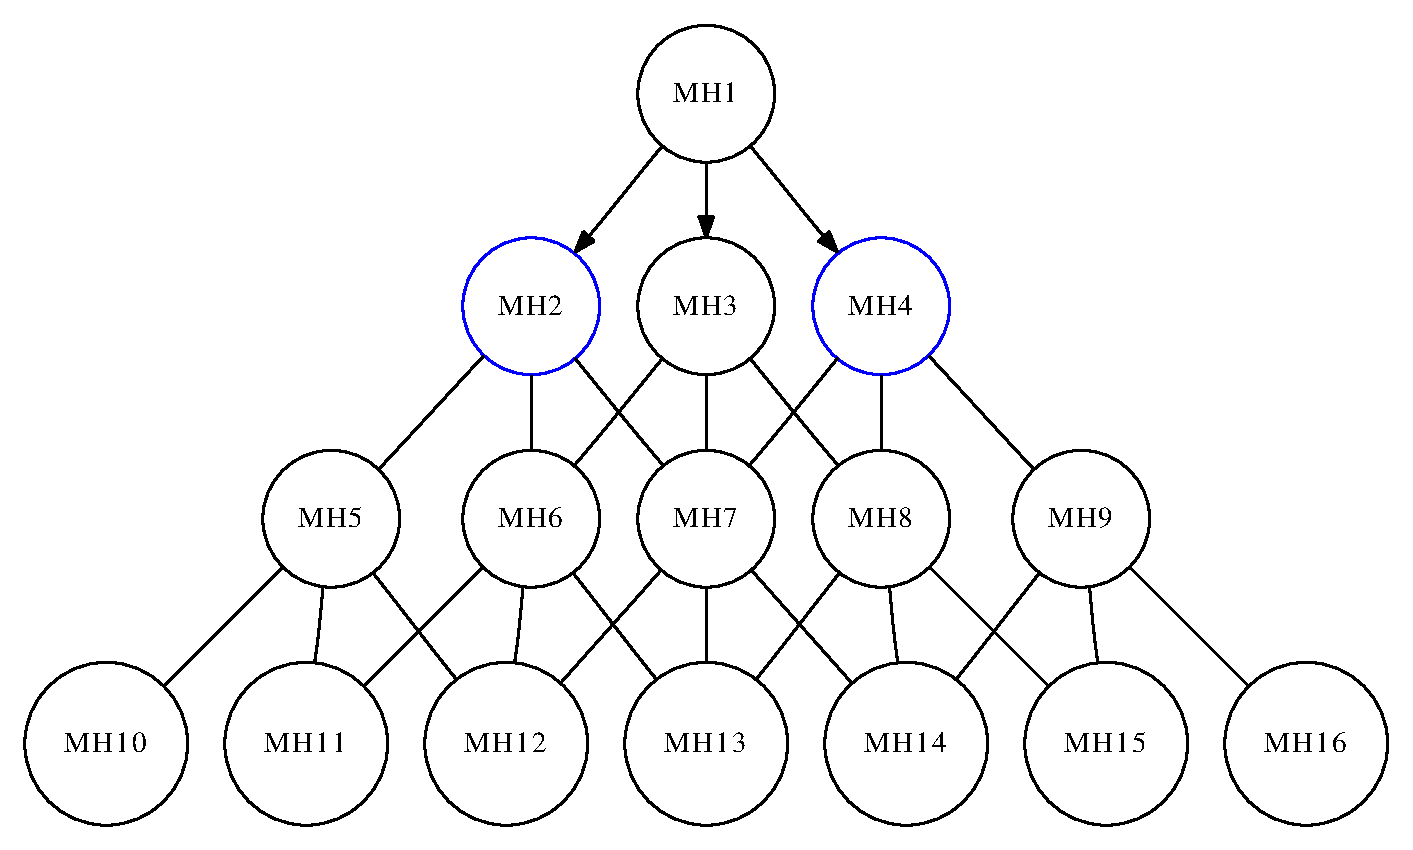
\includegraphics[scale=0.3]{olsrOperationStep5.eps}
	}\label{subfig:olsrStep22}
	\subfigure[Terceiro est\'agio]{
		\includegraphics[scale=0.3]{olsrOperationStep6.eps}
	}\label{subfig:olsrStep23}
	\subfigure[Quarto est\'agio]{
		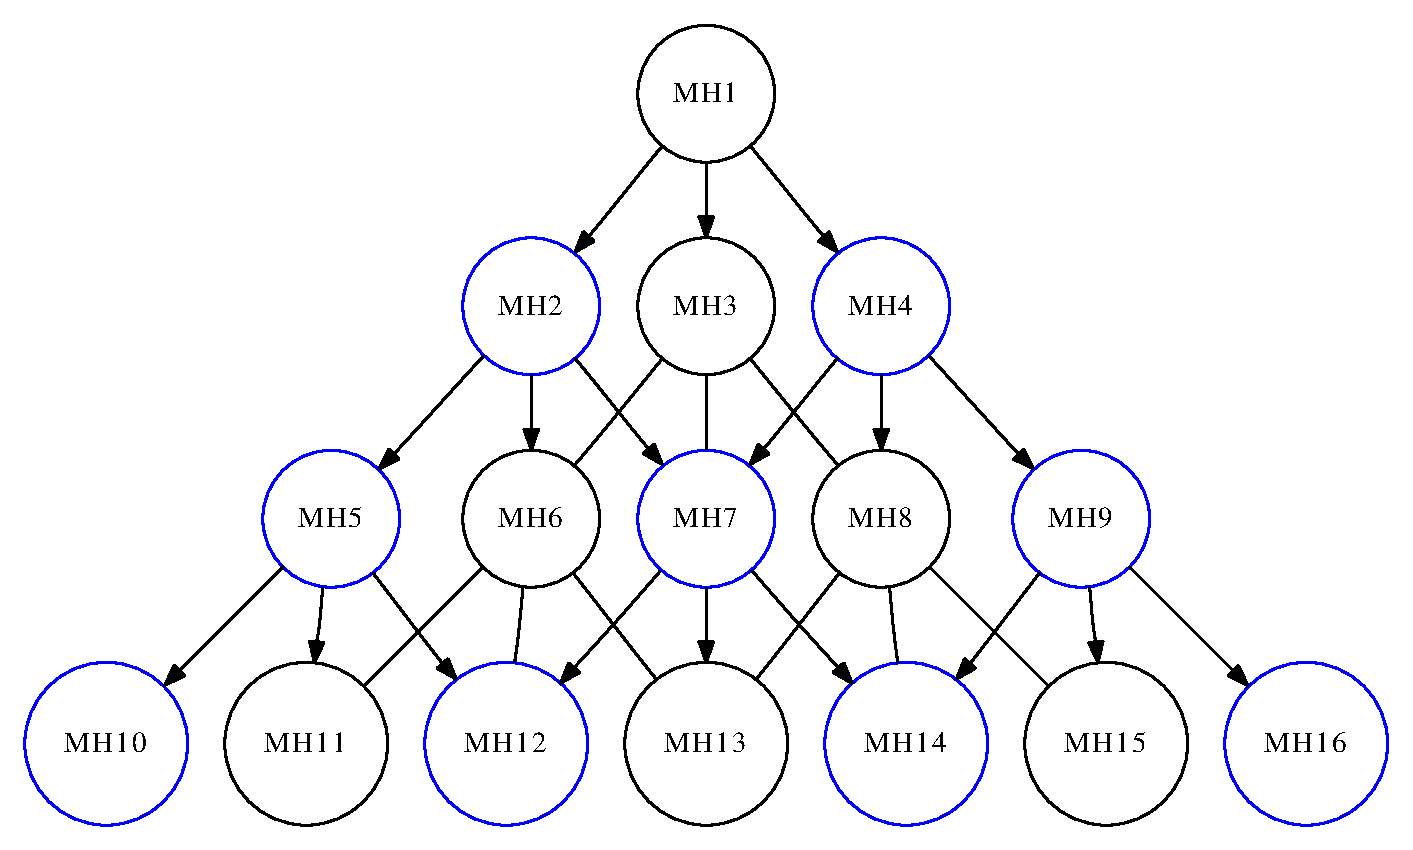
\includegraphics[scale=0.3]{olsrOperationStep7.eps}
	}\label{subfig:olsrStep24}	
	\caption{Descoberta de rotas do protocolo OLSR}
	\label{fig:olsrOperation}
\end{figure}



%\subsubsection{Vantagens do OLSR}
%\begin{itemize}
%	\item Atualiza as rotas no momento em que a topologia da rede altera.
%\end{itemize}

%\subsubsection{Limita\c{c}\~oes e desvantagens do OLSR}
